\chapter{Solutions to the 1D Schr\"odinger Equation}
In one dimension, the time independent Schr\"odinger Equation is
\begin{equation}
    \mathcal{H}\psi=\frac{P^2}{2m}\psi(x)+V(x)\psi(x)=E\psi(x)
\end{equation}
where $\psi(x)$ is the wavefunction, $P$ is the momentum operator, $E$ is the energy eigenvalue, and $V(x)$ is the potential. This equation can be solved exactly for certain potentials. The momentum operator can be written in position space as 
\begin{equation}
P=\frac{\hbar}{i}\frac{d}{dx}    
\end{equation}
The Schr\"odinger equation then becomes
\begin{equation}
    \frac{-\hbar^2}{2m}\frac{d^2 \psi}{dx^2} + V(x) \psi=E\psi
\end{equation}
In the following two sections, the Harmonic Oscillator and the Infinite Well will be considered following the work of Griffiths \cite{Griffiths}.
\section{Harmonic Oscillator}
The harmonic oscillator has a potential that is defined as 
\begin{equation}
    V(x)=\frac{1}{2}m\omega^2 x^2
\end{equation}
Plugging this into the Schr\"odinger equation yields
\begin{equation}
    \frac{-\hbar^2}{2m}\frac{d^2}{dx^2}\psi+\frac{1}{2}m\omega^2 x^2\psi=E\psi
\end{equation}
This can be rewritten as 
\begin{equation}
    E\psi=\frac{1}{2m}\qty[\qty(\frac{\hbar}{i}\frac{d}{dx})^2+\qty(m\omega x)^2]\psi=\mathcal{H}\psi
\end{equation}
To calculate this, I will introduce the following operator
\begin{equation}
    a_{\pm}\equiv \frac{1}{\sqrt{2\hbar m \omega}} (\mp ip+m\omega x)
\end{equation}
The Schr\"odinger equation can be written in terms of this raising and lowering operator. To do so, consider that
\begin{align}
    a_-a_+&=\frac{1}{2\hbar m\omega} (ip+m\omega x)(-ip+m\omega x)\nonumber\\
    &=\frac{1}{2\hbar m\omega} [p^2+(m\omega x)^2-im\omega (xp-px)]\nonumber\\
    &=\frac{1}{2\hbar m\omega} [p^2+(m\omega x)^2]-\frac{i}{2\hbar}[x,p]\nonumber\\
    &=\frac{1}{2\hbar m\omega} [p^2+(m\omega x)^2]-\frac{i}{2\hbar}(i\hbar)\nonumber\\
    &=\frac{1}{2\hbar m\omega} [p^2+(m\omega x)^2]+\frac{1}{2}
\end{align}
where the commutator $[x,p]=xp-px=i\hbar$ was used in the fourth line. $a_-a_+$ can be substituted into Equation (A.6) to arrive at 
\begin{equation}
    \mathcal{H}=\hbar\omega\qty(a_-a_+-\frac{1}{2})
\end{equation}
Some properties of the ladder operators will help later calculations,
\begin{gather}
    [a_-,a_+]=1\\
    a_+\psi_n=\sqrt{n+1} \psi_{n+1}\\
    a_-\psi_n=\sqrt{n}\psi_{n-1}\\
    a_-\psi_0=0
\end{gather}
Using the commutator between the two operators, the Hamiltonian can also be written as 
\begin{equation}
    \mathcal{H}=\hbar\omega\qty(a_+a_-+\frac{1}{2})
\end{equation}
The energy spectrum can be calculated by finding the expectation value of this Hamiltonian. For convenience, let $\psi_n=\ket{n}$. This yields 
\begin{align}
    E=\avg{\mathcal{H}}&=\braket{n|\mathcal{H}|n}=\braket{n|\hbar\omega (a_+a_-+\frac{1}{2})|n}\nonumber\\
    &=\hbar\omega \braket{n|a_+a_-|n}+\frac{\hbar\omega}{2}\braket{n|n}\nonumber\\
    &=\hbar\omega \sqrt{n}\braket{n|a_+|n-1}+\frac{\hbar\omega}{2}\nonumber\\
    &=\hbar\omega n \braket{n|n}+\frac{\hbar\omega}{2}\nonumber\\
    &=\hbar\omega n +\frac{\hbar\omega}{2}\nonumber\\
    &=\hbar\omega(n+\frac{1}{2})
\end{align}
This is the equation for the energy spectrum of the simple harmonic oscillator. It is a linear equation in $n$, so it is called a linear energy spectrum. The energy spectrum can be seen in Figure (A.1).
\begin{figure}
    \centering
    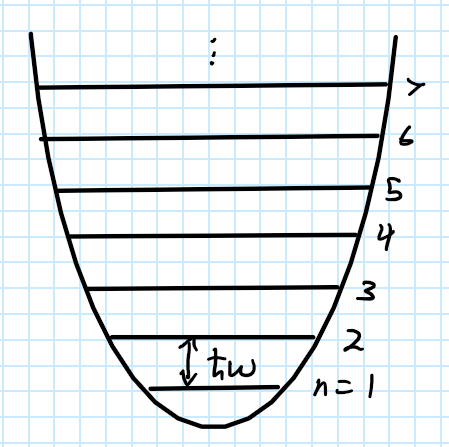
\includegraphics[scale=0.5]{figures/pdf/SHMspectrum.PNG}
    \caption{Simple Harmonic Oscillator Spectrum}
    \label{fig:Simple Harmonic Oscillator Spectrum}
\end{figure}Throughout this paper, any reference to a linear energy spectrum is directly a reference to the energy spectrum of a simple harmonic oscillator. 

\section{Infinite Well}
The infinite square well is defined with a potential 
\begin{equation}
    V(x)=\begin{cases} 0 & 0\leq x \leq a\\
                       \infty & \text{otherwise}
        \end{cases}
\end{equation}
Plotting this potential shows the "well" shape that gives this potential its name. This is shown in Figure (A.2).
\begin{figure}
    \centering
    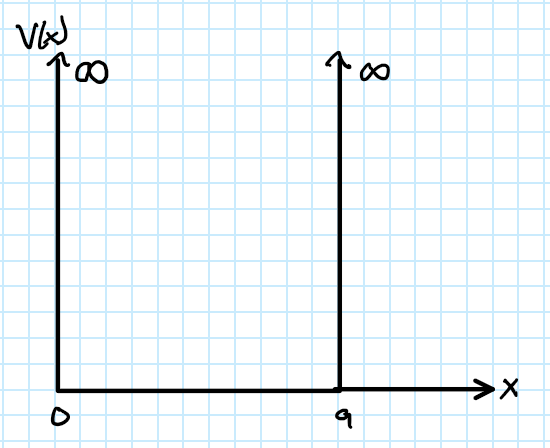
\includegraphics[scale=0.5]{figures/pdf/infsqpot.PNG}
    \caption{Infinite Well Potential}
    \label{fig: Infinite Well Potential}
\end{figure}
When plugging this potential into the Schr\"odinger equation, the only surviving part is when $V=0$. This means that there's one equation to solve with boundary conditions at $x=0,a$. Inserting the potential yields
\begin{align}
    -\frac{\hbar^2}{2m}\frac{d^2\psi}{dx^2}&=E\psi\nonumber\\
    \frac{d^2\psi}{dx^2}&=-\frac{2mE}{\hbar^2}\psi\nonumber\\
    \frac{d^2\psi}{dx^2}&=-k^2\psi
\end{align}
where $k=\frac{\sqrt{2mE}}{\hbar}$. The form of this equation is that of the classical simple harmonic oscillator, so $\psi$ can be directly written as 
\begin{equation}
    \psi=A\sin(kx)+B\cos(kx)
\end{equation}
The boundary condition at $x=0$ gives the $B$ constant 
\begin{align}
    \psi(0)=0&=A\sin(k(0))+B\cos(k(0))\\
    &=0+B\\
    B&=0
\end{align}
The other boundary condition gives
\begin{align}
    \psi(a)=0=A\sin(ka)
\end{align}
The trivial solution to this problem is $A=0$. This does not give any information about the energy spectrum, so instead consider the case where $A\neq 0$. This means that the $\sin(ka)$ term must be zero. This can only happen when $ka=n\pi$ where $n$ is an integer. Since $k$ is related to the energy, the spectrum can be found as
\begin{align}
    k=\frac{\sqrt{2mE}}{\hbar}&=\frac{n\pi}{a}\\
    E&=\frac{1}{2m} \qty(\frac{\hbar n\pi}{a})^2 
\end{align}
Since this equation is quadratic in $n$, it is called the quadratic energy spectrum. The spectrum is shown in Figure (A.3). Any reference to a quadratic spectrum in this paper is considering the energy spectrum in Equation (A.24)
\begin{figure}
    \centering
    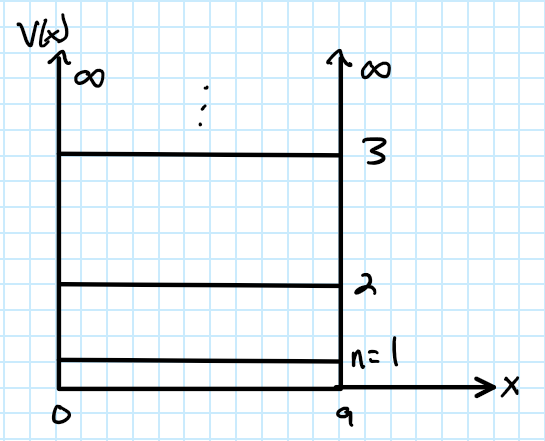
\includegraphics[scale=0.5]{figures/pdf/infsqspec.PNG}
    \caption{Energy spectrum of the infinite square well}
    \label{fig:Energy spectrum of the infinite square well}
\end{figure}
